
\vspace{-10 mm}
\begin{IEEEbiography}[{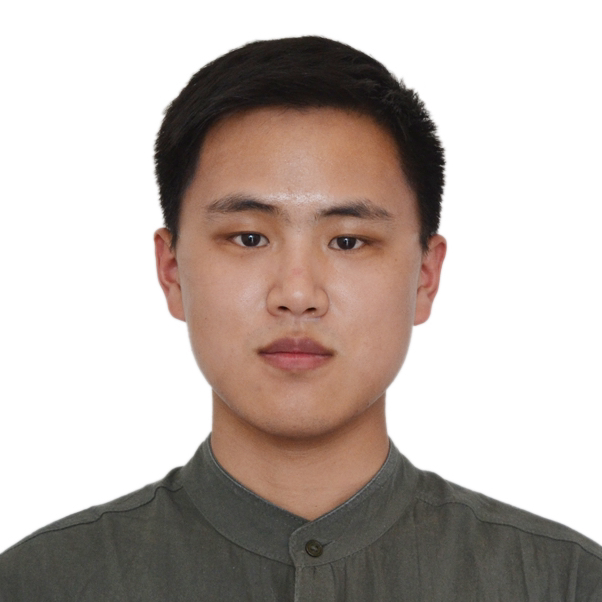
\includegraphics[width=1in,height=1in,clip,keepaspectratio]{./pic/xiangguo}}]{Xiangguo Sun} is a postdoctoral research fellow at the Chinese University of Hong Kong. He was recognized as the "Social Computing Rising Star" in 2023 from CAAI. He studied at  Zhejiang Lab as a visiting researcher in 2022. In the same year, he received his Ph.D. from Southeast University and won the Distinguished Ph.D. Dissertation Award. During his Ph.D. study, he worked as a research intern at Microsoft Research Asia (MSRA) from Sep 2021 to Jan 2022 and won the ''Award of Excellence''. He studied as a joint Ph.D. student at The University of Queensland hosted by ARC Future Fellow Prof. Hongzhi Yin from Sep 2019 to Sep 2021. His research interests include social computing and network learning. He was the winner of the Best Research Paper Award at KDD'23, which is the first time for Mainland and Hong Kong of China. 
% He served as the PC member/reviewer of NeurIPS 2023, The Web Conference (WWW) 2023, SIGIR 2021, ICDE 2021, SIGKDD (2020, 2021, 2022, 2023), VLDB 2022, DASFAA (2020, 2023), TNNLS, etc. 
He has published 11 CORE A*, 9 CCF A, and 13 SCI (including 6 IEEE Trans), some of which appear in SIGKDD, VLDB, The Web Conference (WWW), TKDE, TOIS, WSDM, TNNLS, CIKM, etc.
\end{IEEEbiography}
\vspace{-10 mm}



\begin{IEEEbiography}[{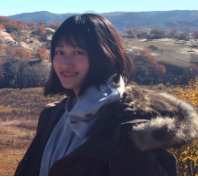
\includegraphics[width=1in,height=1in,clip,keepaspectratio]{./pic/jiawen}}]{Jiawen Zhang} is a Ph.D. student in Data Science and Analytics at HKUST (Guangzhou) under the supervision of Prof. Jia Li. She received her M.Eng. degree in Computer Technology from the Chinese Academy of Sciences. She worked as a research intern at the Machine Learning Group in Microsoft Research Asia. Her research interests include data mining and time series modeling.
\end{IEEEbiography}
\vspace{-13 mm}

\begin{IEEEbiography}[{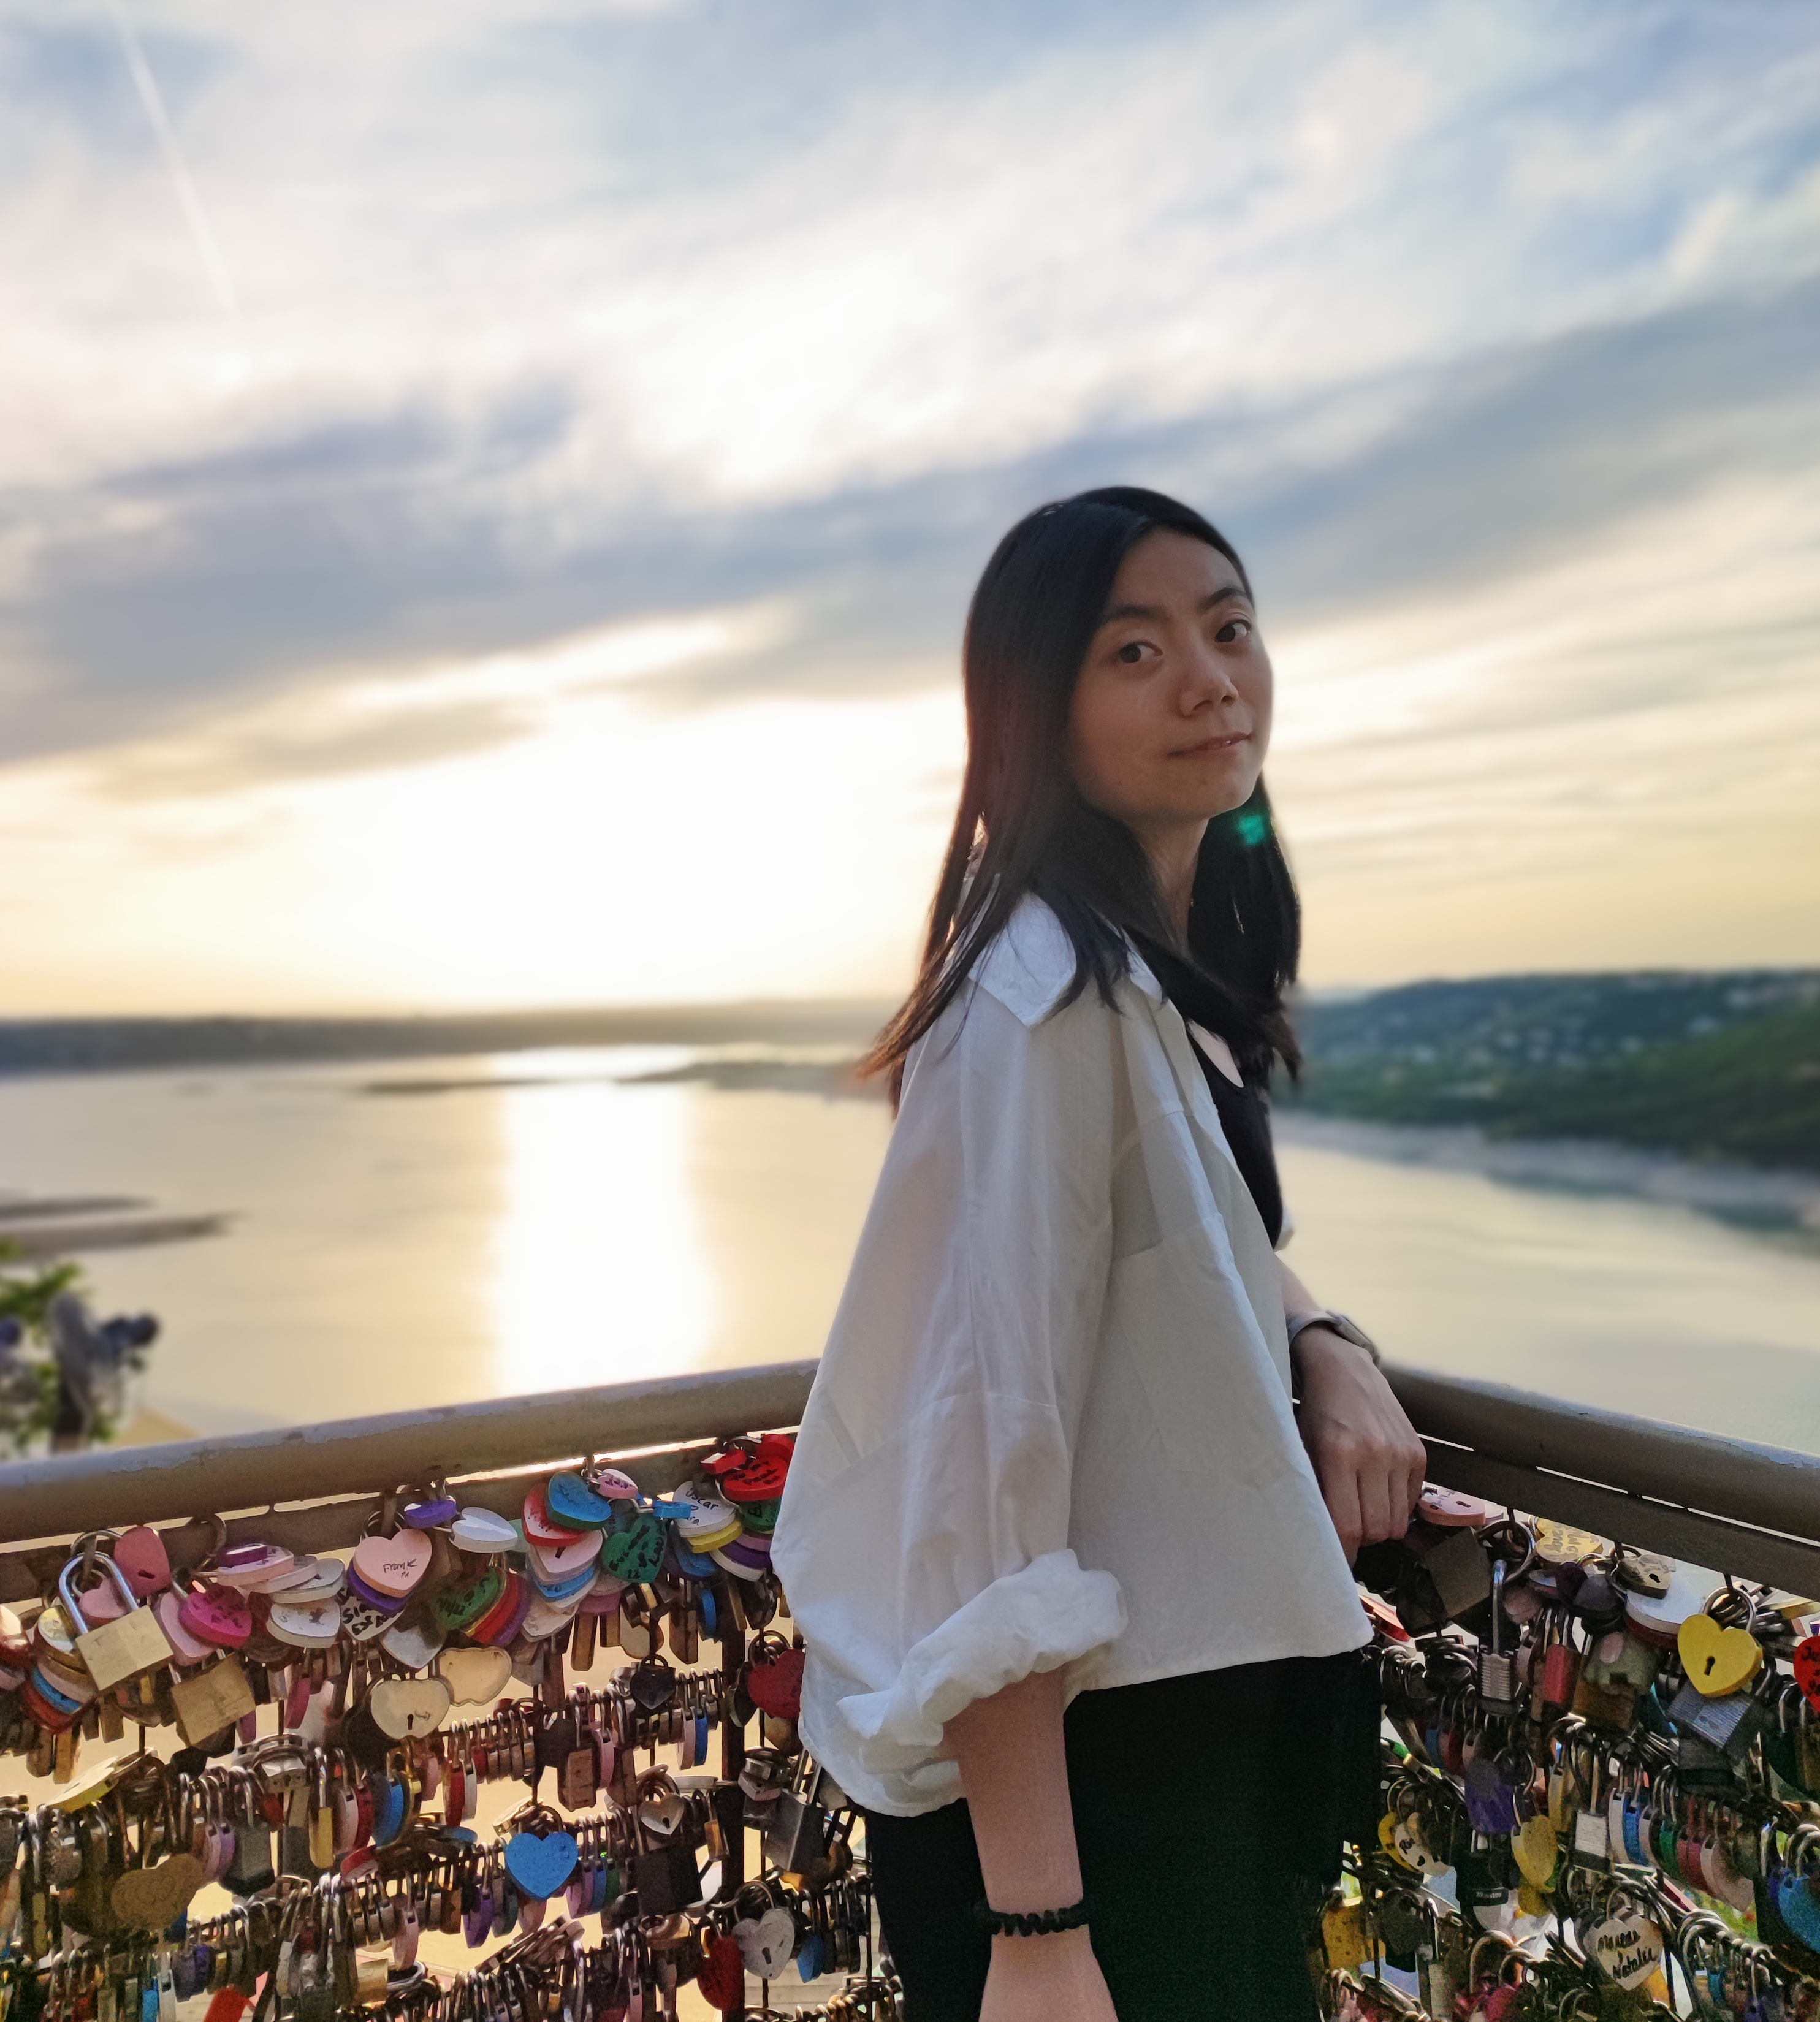
\includegraphics[width=1in,height=1in,clip,keepaspectratio]{./pic/xixi}}]{Xixi Wu} is a final-year master student at School of Computer Science, Fudan University. She obtained her B.S. in Computer Science from Fudan University in 2021. Her research interests include Deep Graph Learning, Data Mining, and Recommender Systems. She has published multiple first-authored papers at KDD/WWW/CIKM.
\end{IEEEbiography}
\vspace{-13 mm}



\begin{IEEEbiography}[{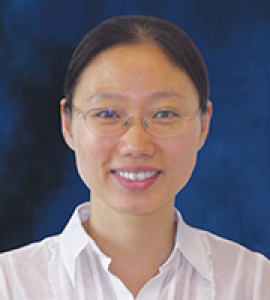
\includegraphics[width=1in,height=1in,clip,keepaspectratio]{./pic/hongcheng}}]{Hong Cheng} is a Professor in the Department of Systems Engineering and Engineering Management, Chinese University of Hong Kong. She received the Ph.D. degree from the University of Illinois at Urbana-Champaign in 2008. Her research interests include data mining, database systems, and machine learning. She received research paper awards at ICDE'07, SIGKDD'06, and SIGKDD'05, and the certificate of recognition for the 2009 SIGKDD Doctoral Dissertation 
 Award. She received the 2010 Vice-Chancellor's Exemplary Teaching Award at the Chinese University of Hong Kong.
\end{IEEEbiography}
\vspace{-10 mm}

\begin{IEEEbiography}[{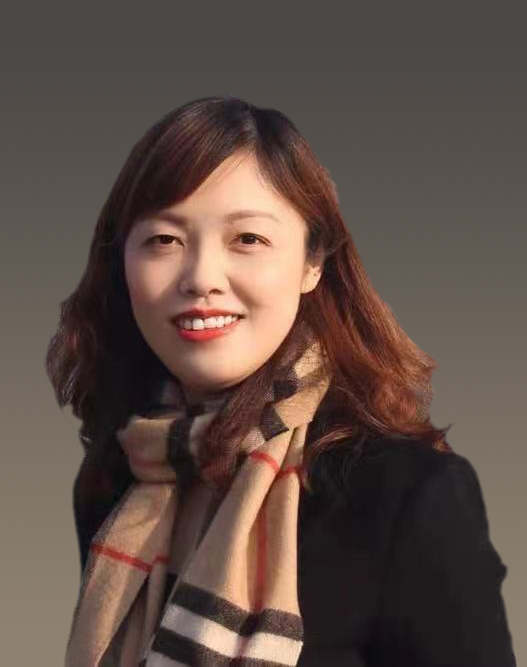
\includegraphics[width=1in,height=1in, clip,keepaspectratio]{./pic/yunxiong.jpg}}]{Yun Xiong} is a Professor in Shanghai Key Laboratory of Data Science, School of Computer Science, Fudan University. She obtained her Ph.D. degree from Fudan University in 2008. Her research interests include big data mining and data science. Her research achievements include the publication of more than 50 papers in internationally top journals and conferences in the field of Data Mining, including TKDE, KDD, WWW, AAAI, etc.
\end{IEEEbiography}
\vspace{-13 mm}

\begin{IEEEbiography}[{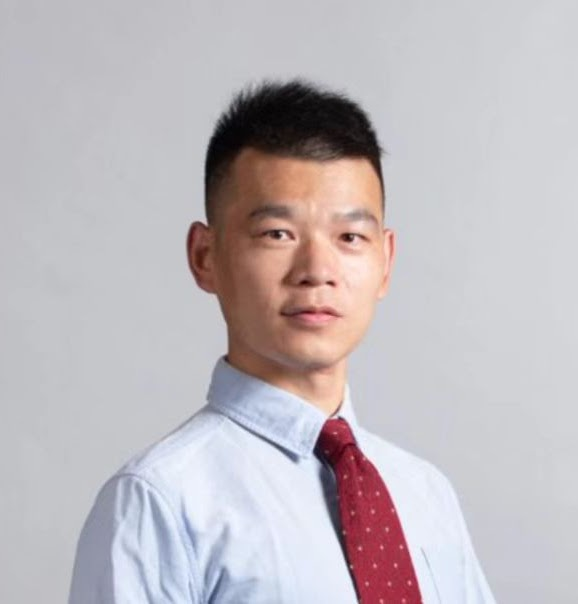
\includegraphics[width=1in,height=1in,clip,keepaspectratio]{./pic/jiali}}]{Jia Li} is an assistant professor in HKUST (Guangzhou). He received Ph.D. degree at The Chinese University of Hong Kong in 2021. Before that, he worked as a full-time data mining engineer at Tencent from 2014 to 2017, and research intern at Google AI (Mountain View) in 2020. His research interests include graph learning and data mining. Some of his work has been published in TPAMI, ICML, NeurIPS, WWW, KDD, etc.
\end{IEEEbiography}


\vfill